\chapter{Estado del arte}
\label{cap:capitulo2}
	
En el presente capítulo, se van a describir algunos de los prototipos y soluciones más destacables aplicadas a la detección y recolección de fresas usando inteligencia artificial y técnicas robóticas.

En los sistemas de producción de cultivos, hay operaciones de campo que requieren mucha mano de obra, ya sea por su complejidad o por el hecho de que están relacionadas con una interacción sensible entre plantas y productos comestibles, o por la repetitividad que requieren a lo largo de un ciclo de producción de cultivos. Estos son los factores clave para el desarrollo de robots agrícola, tal y como se relata en el artículo \cite{Fountas20}, donde se realiza una revisión sistemática de la bibliografía existente sobre la investigación y la robótica agrícola comercial utilizada en las operaciones de los campos de cultivo en función de las principales operaciones de campo, siendo estas: deshierbe, siembra, detección de enfermedades e insectos, exploración de cultivos (seguimiento de plantas y fenotipado), pulverización o rociado, cosecha, robots de gestión de plantas y sistemas robóticos polivalentes.

\begin{figure} [H]
    \begin{center}
      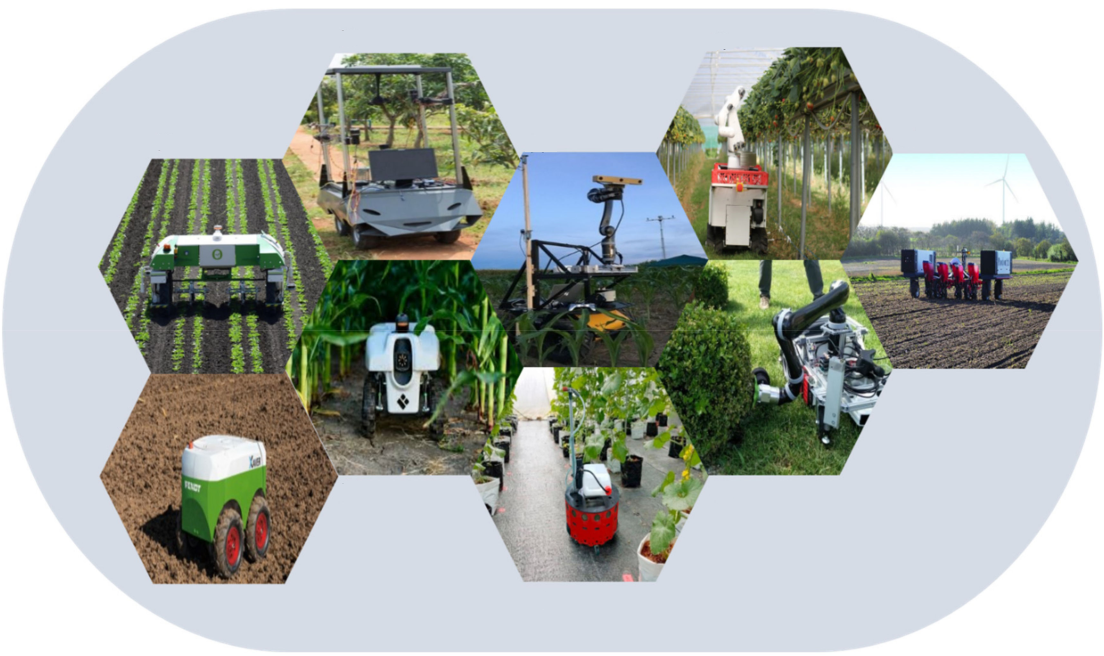
\includegraphics[width=12cm]{figs/Representación robots agrícolas.png}
    \end{center}
    \caption{Representación de varios tipos de robots agrícolas}
    \label{fig:Robots_agricolas}
\end{figure}

Entre estas operaciones se escogió centrarse en la recolección, que es una de las tareas más laboriosas y repetitivas, a la vez que forma parte de todos los ciclos de producción en la agricultura, existiendo dos tipos de cosechadoras robotizadas: a granel (se recogen todas las frutas/verduras) y selectivas (sólo se recogen las frutas maduras/listas para ser cosechadas) \cite{Fountas20}, dentro de las cuales se engloba este trabajo final de grado. 

La mayoría de los robots de recolección se centran en las fresas, un cultivo de alto valor, que sufre un alto coste de producción debido principalmente al coste de la mano de obra, sobre todo durante la recolección. Los robots de recolección de fresas más rápidos fueron los robots con velocidades de recolección de 7,5 y 8,6 segundos por fresa, respectivamente, y el robot Berry 5 de Harvest Croo \footnote{\url{https://www.harvestcroorobotics.com/}}, con una velocidad de recolección declarada de 8 segundos por fruta. 

Sin embargo, no basta con tener una alta velocidad de recogida, ya que también es importante una alta tasa de recogida, siendo la más alta presentada del 86\%. 
Para evaluar el rendimiento de los robots en la recolección, se ha mostrado un rango en las tasas de éxito de recolección, desde el 0\% hasta el 64\%, para varias categorías, tal y como se muestra en la ilustración de la Figura \ref{fig:RendimientosCosecha}, mereciendo la pena mencionar que para la recolección de fresas, parece haber un equilibrio entre la velocidad y la tasa de recolección, ya que las velocidades de recolección rápidas van acompañadas de tasas de recolección bajas y viceversa \cite{Fountas20}. 

\begin{figure} [H]
    \begin{center}
      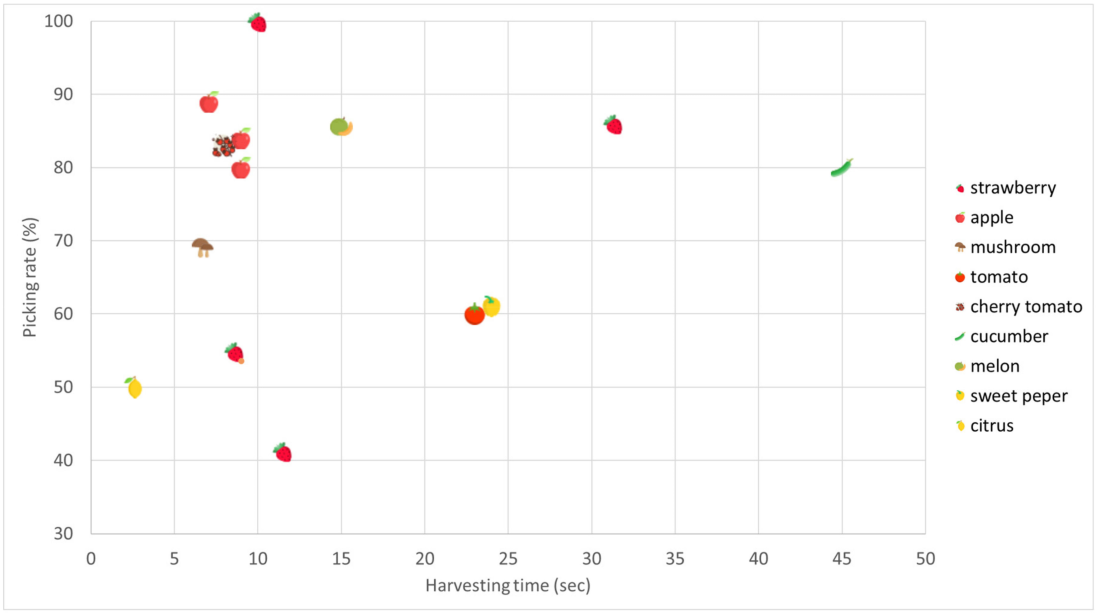
\includegraphics[width=15cm]{figs/Rendimiento cosecha robots.png}
    \end{center}
    \caption{Ilustración global del rendimiento general de los robots revisados}
    \label{fig:RendimientosCosecha}
\end{figure}

En 2009, después de más de 30 años de comercializar fresas en la provincia de Huelva, y de algunos intentos infructuosos, la empresa AGROBOT \footnote{\url{https://www.agrobot.com/?lang=es}}, con sede en el Centro de Innovación y Tecnología que la Consejería de Innovación tiene en Lepe (Huelva), consiguió poner en marcha un prototipo con 40 brazos robóticos que identificaba los frutos maduros y los recogía sin dañarlos, siendo capaz de clasificarlas y colocarlas en los envases que recorren las cintas transportadoras, gracias a un grupo de ingenieros liderado por Juan Bravo \cite{Cabanillas09}. Tras la presentación del prototipo y las primeras pruebas con éxito, la empresa onubense desarrolló el prototipo final, el Agrobot SW 6010, una cosechadora de fresas que es capaz de recoger de la mata solo la fruta que está madura mediante inteligencia artificial con 30 brazos robóticos que incorporan una cámara con visión artificial que detecta el grado de madurez de la fruta. Recopila entre 10 y 30 imágenes por segundo, permitiendo a los algoritmos confirmar, mediante un análisis morfológico y de color en tiempo real, si la fresa cumple con los parámetros marcados de tamaño, grosor y color. Si la fresa está verde se quedará en la planta, siendo la robótica quien corta el tallo de la fruta y la deposita en una cinta transportadora para que posteriormente sean los humanos quienes clasifiquen las fresas y las guarden en las cajas para su distribución \cite{Maite19}. Este modelo se volvería a mejorar para obtener el Agrobot E-Series \footnote{\url{https://www.agrobot.com/e-series}} (Figura \ref{fig:Agrobot}), que consta de hasta 24 brazos robóticos independientes, permitiendo adaptarse a cualquier configuración agrícola, y que, fabricado en acero inoxidable y aluminio de calidad militar, puede funcionar de forma robusta con un alto grado de precisión, ya que su arquitectura de brazos descentralizada y autosuficiente hace que sea especialmente fácil de configurar y mantener, y los sensores de profundidad infrarrojos y en color integrados de corto alcance a bordo, que surven para captar todos los detalles están respaldados por unidades de procesamiento gráfico, que ayudan a evaluar el grado de madurez de la fruta, incorporando a su vez, sensores LiDAR que se encargan de la seguridad de los trabajadores del campo circundantes.

\begin{figure}[H]
    \begin{center}
      \subcapcentertrue
      \subfigure[Agrobot E-Series]{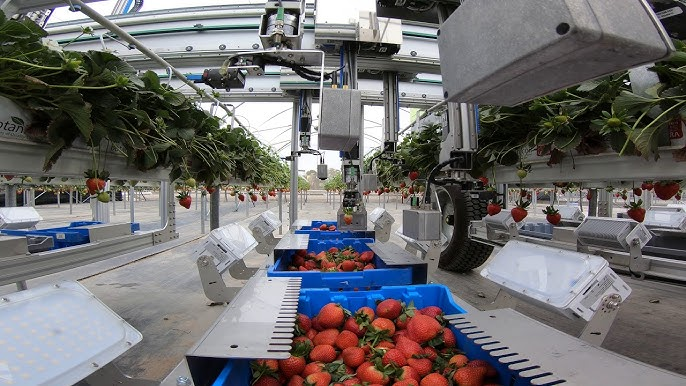
\includegraphics[width=7cm]{figs/Agrobot.jpg}}
      \hspace{2mm}
      \subfigure[Representación 3D del Agrobot E-Series]{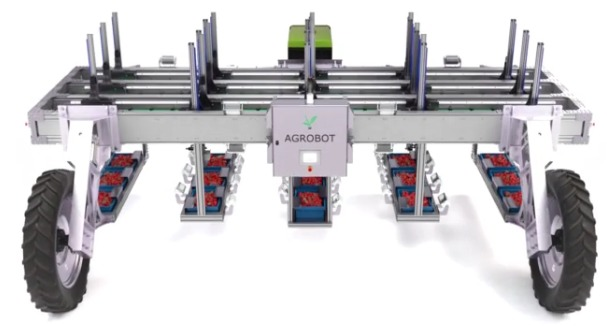
\includegraphics[width=7cm]{figs/Agrobot 3D.png}}
    \end{center}
    \caption{Agrobot}
    \label{fig:Agrobot}
  \end{figure}

La empresa belga de I+D agrícola Octinion \footnote{\url{http://octinion.com/products/agricultural-robotics/rubion}} desarrolló un prototipo de robot recolector de fresas en 2017, que recoge los frutos de forma totalmente autónoma basándose en el método de cultivo habitual (sobremesa), con el fin de resolver el obstáculo emergente de la agricultura occidental: la falta de mano de obra asequible que pone en peligro la sostenibilidad y conservación del negocio \cite{DePreter18}.

Este robot, cuyo diseño está representado en la Figura \ref{fig:DiseñoConceptual_Octinion}, está formado por un vehículo eléctrico consistente en una plataforma eléctrica con una batería recargable; un sistema de localización consituido por codificadores de rueda, un giroscopio y un sistema de posicionamiento en interiores de banda ultraancha (UWB); tres cámaras RGB utilizadas para la detección de las fresas por cámara mediante visión artificial, un brazo robótico diseñado a medida, la pinza que se acopla al extremo del brazo robótico y agarra con sus dedos la fresa detectada, un módulo de gestión o manipulación logística consistente en varias cestas que se transportan en la plataforma eléctrica y que están preparadas por el robot para que estén inmediatamente listas para el envasado final y el transporte; y un módulo de control de calidad que clasifica las fresas detectadas en función de su madurez, forma, tamaño y dulzor \cite{DePreter18}.

\begin{figure} [H]
    \begin{center}
      \includegraphics[width=13cm]{figs/DiseñoConceptual_Octinion.png}
    \end{center}
    \caption{Diseño conceptual del robot de recogida con sus componentes}
    \label{fig:DiseñoConceptual_Octinion}
\end{figure}

Todo esto le permite al robot recoger al menos el 70\% de las fresas maduras, siempre sin dañarlas, ya que sólo decide recoger la fruta si su acción no va a dañar otras fresas, siendo el tiempo necesario para desplazarse hasta la fresa, cogerla y depositarla en una cesta (caja en la que se colocan las
fresas) de 4 segundos, siendo la calidad y velocidad de recolección comparables a las de un recolector humano ideal \cite{DePreter18}. Además de esto, el uso de este robot para cosechar las fresas de forma autónoma, presenta algunas ventajas adicionales:

\begin{itemize}
    \item Mayor calidad de recolección (disminución de los daños en la fruta).
    \item Mayor calidad de clasificación (más categorías, colocación más óptima 								en los envases, categorización mejor y más flexible).
    \item La productividad del robot es constante y predecible. No necesita formación, por lo que no supone un coste elevado al principio.
    \item Nuevas herramientas de gestión con los datos recopilados: predicción del rendimiento, asignaciones de cosecha más complejas (recogida de un tamaño
determinado, recogida un día antes o después).
    \item Horario de recogida ilimitado (fines de semana, horario nocturno).
\end{itemize}

El sistema Dogtooth \footnote{\url{https://dogtooth.tech/}} de Cambridge (Reino Unido) (ver en Figura \ref{fig:Dogtooth}) fue desarrollado para mejorar las operaciones de recogida de frutos rojos siendo capaz de navegar por hileras de fresas y frambuesas, detectar y localizar las maduras, así como recoger y comprobar la fruta antes de colocarla en un cesto, permite a las empresas de recolección de fruta sustituir el método de recogida manual y ahorrar tiempo. Sin embargo, al cortar el tallo produce una pequeña herida, que permite que las enfermedades entren fácilmente en la planta, y la parte restante del pedúnculo puede magullar otras fresas durante el transporte, cuando las frutas se agitan en sus cajas. Así mismo, Dogtooth parte de un robot industrial caro cuya cinemática no está optimizada para la recogida de fresas, suponiendo un inconveniente frente a sus competidores que, a pesar de encontrarse en fase de prototipo, sus conceptos exigen cambios drásticos en la infraestructura ya que las fresas recolectadas no cumplen las especificaciones exigidas por el mercado. 

\begin{figure}[H]
    \begin{center}
      \subcapcentertrue
      \subfigure[Robot Dogtooth]{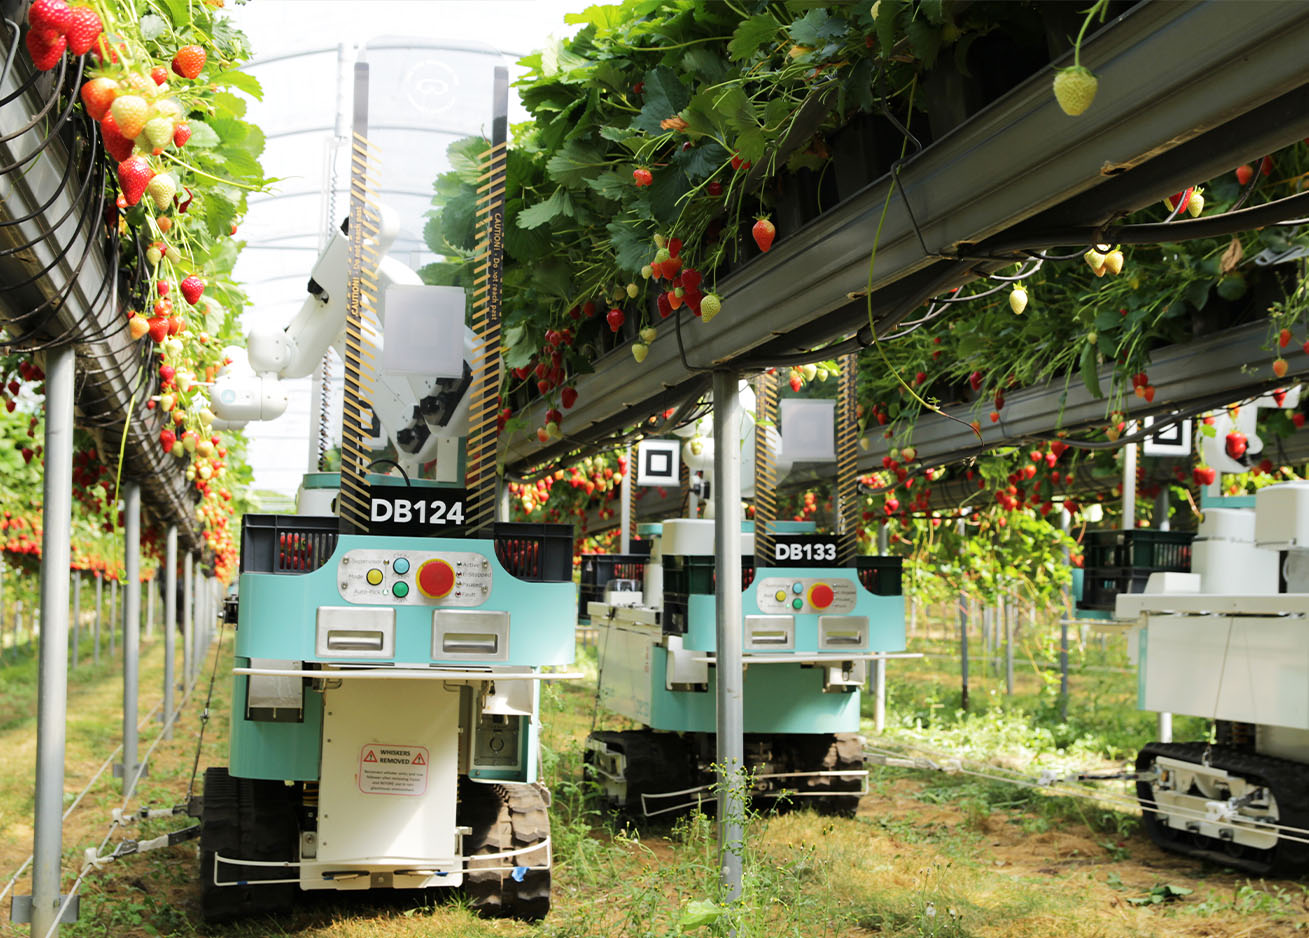
\includegraphics[width=12cm]{figs/Dogtooth.jpg}}
      \hspace{2mm}
      \subfigure[Brazo robótico del Dogtooth]{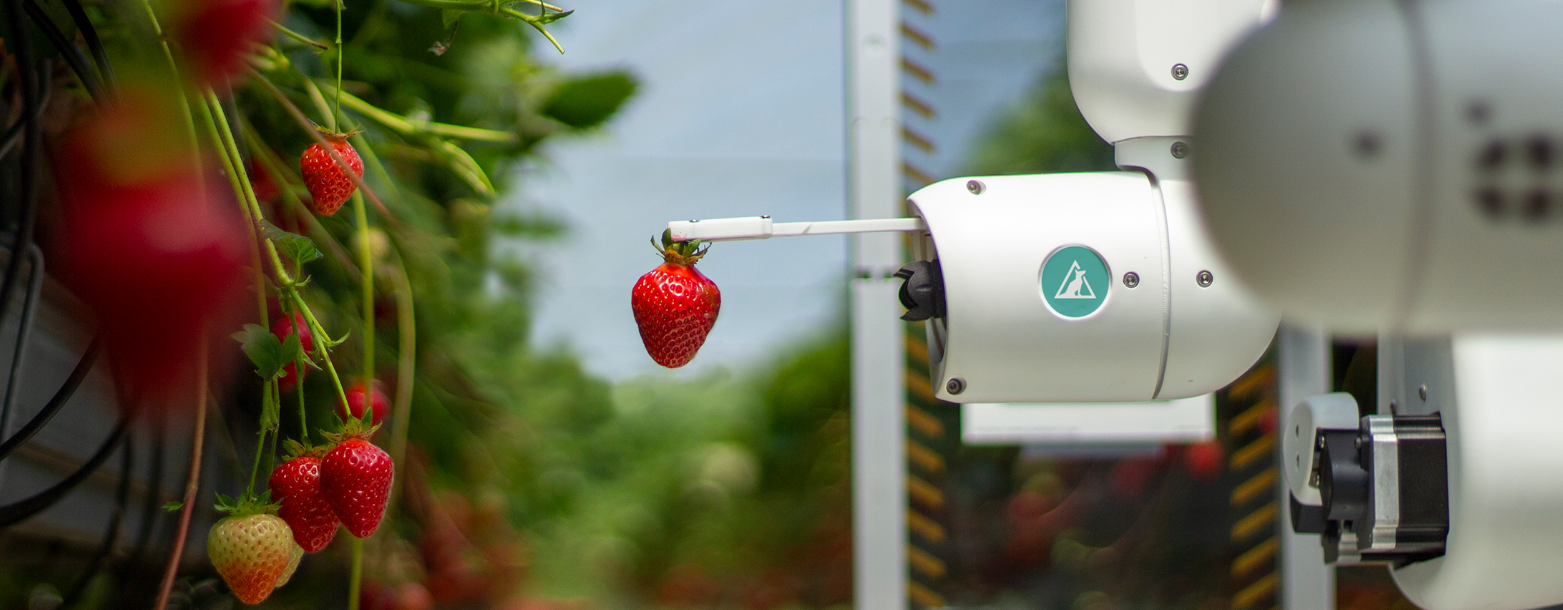
\includegraphics[width=12cm]{figs/Brazo Dogtooth.png}}
    \end{center}
    \caption{Robot agrícola Dogtooth}
    \label{fig:Dogtooth}
\end{figure}

El sistema explicado en \cite{Xiong19}, presenta el desarrollo y la evaluación de un robot para la recolección de fresas (Fragaria × ananassa) cultivadas en invernaderos (ver Figura \ref{fig:Robot_Xiong}). El robot encargado de realizar esta tarea, está compuesto por una pinza montada en un brazo industrial que a su vez está montado en una base móvil junto con una cámara RGB-D, que utilizará el sistema de visión que se basa en el umbral de color combinado con el cribado del área del objeto y el rango de profundidad para seleccionar las fresas maduras y alcanzables. La novedosa pinza está diseñada para apuntar a la fruta y no al tallo, por lo que sólo requiere la ubicación de la fruta para la recolección. Además, está equipada con sensores internos, por lo que la pinza puede detectar y corregir errores de posición, y es resistente a los errores de localización introducidos por el módulo de visión. Otra característica importante de la pinza es el contenedor interno que se utiliza para recoger las bayas durante la recolección, lo cual reduce considerablemente el tiempo de recogida dado que el manipulador no tiene que ir y venir entre cada fresa a una cesta separada.

\begin{figure} [H]
    \begin{center}
      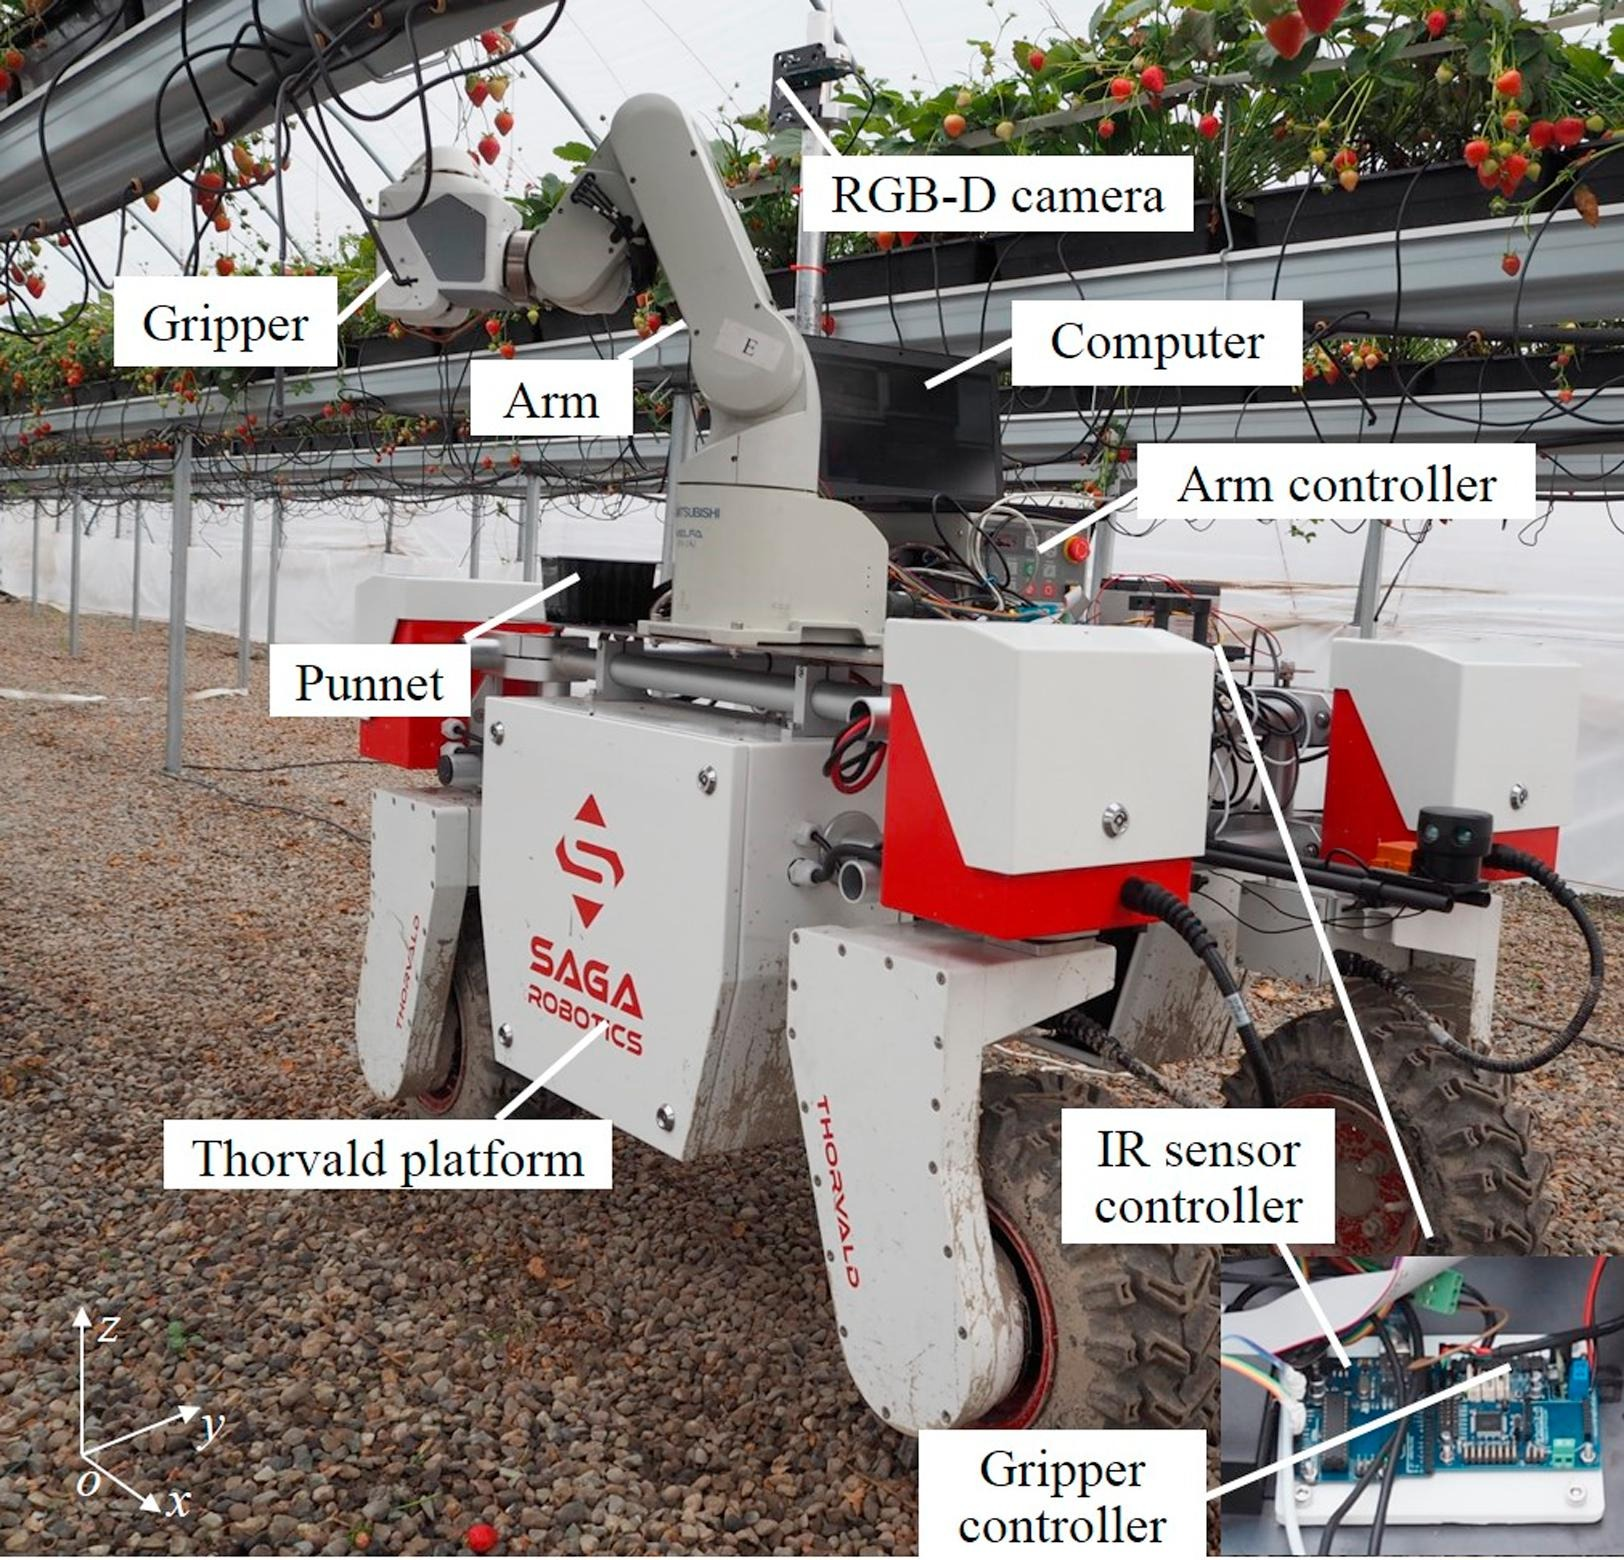
\includegraphics[width=8cm]{figs/Hardware assembly in a strawberry farm.jpg}
    \end{center}
    \caption{Montaje del hardware en una explotación de fresas: el robot consta principalmente de una cámara RGB-D, un brazo 5-DOF, una pinza y una plataforma móvil}
    \label{fig:Robot_Xiong}
\end{figure}

Con todo esto, los experimentos de campo muestran la duración media del ciclo de recolección continua de una sola fresa es de 7,5 s y de 10,6 s cuando se incluyen todos los procedimientos. Además, el robot es capaz de recoger fresas aisladas con una tasa de éxito cercana a la perfección (96,8\%). Sin embargo, en las explotaciones agrícolas, el porcentaje medio de éxito es del 53,6\%, y del 59,0\% si se incluye el «éxito con daños». \\

Este descenso de la tasa de éxito es debido a los siguientes factores:

\begin{itemize}
    \item Oclusión de las fresas, lo que deriva en una detección fallida y una no recolección de las mismas
    \item Posibles detecciones duplicadas debido a las agrupaciones de fresas que se tocan entre sí
    \item Errores de localización demasiado grandes para la que la pinza pueda coger la fresa producidos por localizaciones imprecisas y/o fallos de segmentación del sistema de visión artificial
    \item Perturbaciones que produce la pinza cuando se encuentran fresas por debajo del objetivo o dentro del área de búsqueda de la pinza, por lo que la pinza detecta las fresas molestas y las considera objetivos. También debido a los toques que pueda tener el brazo robótico durante el proceso de recolección con las plantas, ya que estos tpques afectan a la ubicación de objetivos.
    \item Región de alcance del robot reducida, ya que el espacio de trabajo con el que cuenta el brazo robótico para llevar a cabo la tarea de recolección es limitado
    \item Fallos de comunicación del brazo o la pinza
\end{itemize}

En 2020, la Universidad Politécnica Negeri Sriwijaya de Indonesia, analizó desde el departamento de ingeniería eléctrica, el empleo de un robot recolector como proyecto piloto, tal y como se cuenta en el artículo \cite{Oktarina20}, en el cual la fruta a recolectar serían tomates rojos y verdes, en lugar de fresas. A pesar de la diferencia en el tipo de cultivo, el estudio resulta relevante para este trabajo debido a la similitud en los principios de detección y recolección de frutos, y al tratarse de un prototipo básico lo convierte en un punto de partida útil para proyectos de investigación enfocados en la automatización agrícola aplicada a fresas.\\

El objetivo de este estudio es establecer el proyecto inicial en la creación de una serie de robots aplicados en la agricultura para hacer realidad la idea de la agricultura digital. La novedad de este estudio es que este método es simple, al igual que el procesamiento de imágenes, para adaptarse a los recursos limitados de los procesadores con los que se llevó a cabo este proyecto. El robot diseñado se personaliza en función del tamaño de la tomatera y el color, donde la ubicación del tomate se indica mediante un círculo resultante del tratamiento de la imagen y la división en las posiciones izquierda, derecha y central en el plano de la imagen, cuya resolución en este estudio es de 320 × 180 píxeles, como se muestra en la Figura \ref{fig:Deteccion_tomates}. 

\begin{figure}[H]
    \begin{center}
      \subcapcentertrue
      \subfigure[Detección de tomates rojos]{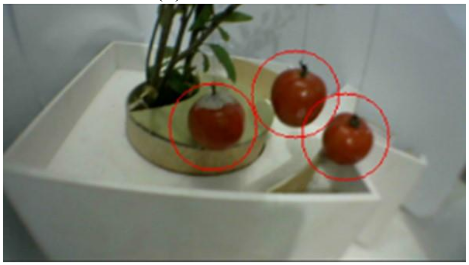
\includegraphics[width=7cm]{figs/Tomate rojo.png}}
      \hspace{2mm}
      \subfigure[Detección de tomates verdes]{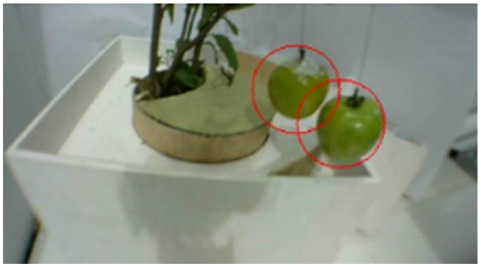
\includegraphics[width=7cm]{figs/Tomate verde.png}}
    \end{center}
    \caption{Detección de tomates indicada por los círculos rojos}
    \label{fig:Deteccion_tomates}
  \end{figure}

El robot, representado en la Figura \ref{fig:Robots_tomates}, consta de una cámara web común instalada en el efector final y un sensor ultrasónico de proximidad HC-SR04 que puede detectar desde 2 cm hasta 400 cm, con un ángulo de detección de hasta 30º como entradas, siendo la cámara quién captura la imagen en bruto de la fruta, mientras que el sensor de proximidad detecta la distancia entre el efector final, que consiste en una tijera para cortar la rama de tomates, y la fruta objetivo. El procesamiento de la imagen en bruto de la cámara se lleva a cabo en el procesador principal, que para este caso es un Arduino Mega 2560, y el resultado del procesamiento de imágenes (los tomates detectados) se envían a la Raspberry Pi 3 Modelo B, donde estos dan el número binario «1» correspondiente a los tomates detectados, mientras que al resto de la imagen, convertida en escala de grises, se considera «0», y se envían al microcontrolador los ángulos de los servomotores que mueven el robot para acercarse a los tomates. Este brazo robótico es un robot con 4 grados de libertad, formado por un servomotor para la base, dos articulaciones y un efector final, donde los servomotores están conectados a las articulaciones y al efector final, y el sensor de proximidad acoplado al efector final proporciona la información al microcontrolador para garantizar la distancia de recogida correcta entre el efector final y los tomates.\\

\begin{figure}[H]
    \begin{center}
      \subcapcentertrue
      \subfigure[Conexión eléctrica entre los componentes del robot recolector]{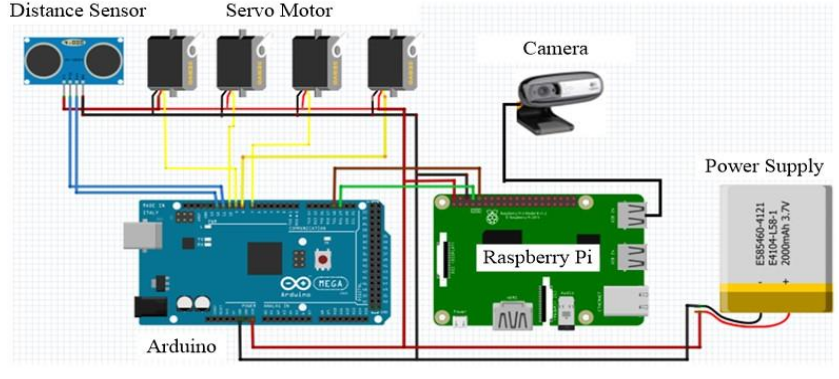
\includegraphics[width=11.5cm]{figs/Componentes recolector tomates.png}}
      \hspace{2mm}
      \subfigure[Diseño tridimensional del robot recolector]{\includegraphics[width=11.5cm]{figs/Diseño 3D recolector tomates.png}}
    \end{center}
    \caption{Robot recolector de tomates}
    \label{fig:Robots_tomates}
\end{figure}

Con todo esto, obtenemos un tiempo medio de recolección del tomate rojo de 4,932 s, y del tomate verde de 5,276 s, siendo el tiempo necesario para que el robot detecte el tomate rojo y vuelva a la posición de espera de 9,676 s, y de 10,586 s para los tomates verdes. Esta diferencia de tiempo se debe a la distancia del robot al tomate y no al color del mismo.







